To lay the foundation for the subsequent \gls{mor} approach, we begin by deriving the \textit{parametric formulation} of transient flow problems defined in deforming domains. As mentioned before, parametric problems, e.g., may occur in the context of \gls{uq} or automatic control. Specifically, we consider problems that can be parametric in the \textit{material properties} involved or in their \textit{boundary conditions}. The variations in the material illustrate potential uncertainties in the process under investigation, which may be analyzed using \gls{uq}. Apart from that, adjustable boundary conditions prescribing, e.g., the inflow velocity, showcase the type of use in a context such as automatic control. 
As mentioned earlier, we focus on unsteady processes that take place in time-varying domains, which potentially undergo topology changes, too.

\bigskip\par
For the description of the time-dependent solution field in a deforming domain, it is convenient to treat space and time coordinates, which are denoted by $\x$ and $t$, in the same way. To that end, the \textit{time-continuous space-time domain} $\domainSpaceTime$ is introduced, which results from the time-dependent spatial domain $\domainSpace(t)$ and the time interval $[0,T]$:
\begin{align}
\domainSpaceTime = \domainSpace(t) \times [0,T],    
\end{align}
such that $(\x,t) \in \domainSpaceTime$. The respective space-time boundary is denoted as $\boundarySpaceTime$ where portions on which conditions of Dirichlet or Neumann type are prescribed are referred to as $\boundarySpaceTimeDirichlet$ and $\boundarySpaceTimeNeumann$, respectively.  Furthermore, initial conditions can be imposed over $\domainSpace(t=0)=\domainSpace(t_0)$. A sketch can be found in \Cref{fig:cst}. In contrast, in a \textit{time-discontinuous space-time} approach, one considers so-called time slabs $\domainSpaceTime_m$ with boundaries $\boundarySpaceTime_m$(see \Cref{fig:dst}). This results in a kind of time-stepping scheme with a modified computational domain in each time step. In that sense, the time-discontinuous approach is comparable to a semi-discrete description. A systematic comparison of time-continuous and time-discontinuous space-time formulations for advection-diffusion problems can be found in ~\cite{Danwitz2022}. However, as we would like to stress again, the time-continuous description is essential to directly apply established \gls{mor} techniques for deforming domain problems later.
\begin{figure}
    \centering
    \subcaptionbox{The time-continuous approach.\label{fig:cst}}{
    \newcommand*\cols{2}
\newcommand*\rows{2}
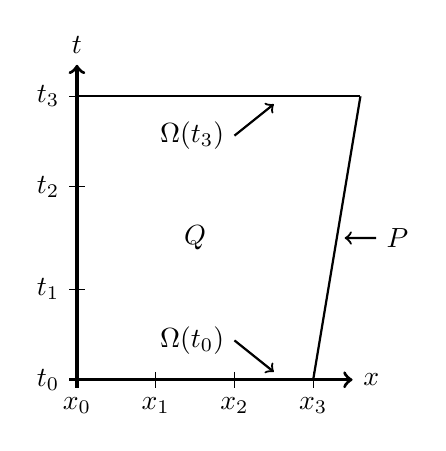
\begin{tikzpicture}[
    scale=1,
    axis/.style={very thick, ->},
    important line/.style={thick},
    every node/.style={color=black}
    ]
    %x-axis
    \draw[axis] (-0.1,0)  -- (3.5,0) node(xline)[right]{$x$};
    \foreach \x in {0,1,2,3}
    \draw (\x cm,0.1) -- (\x cm,-0.1) node[anchor=north] {$x_{\x}$};
    % t-axis
%    \draw[very thick] (0,-0.1) -- (0,1);
%    \draw[very thick] (0,1.3) -- (0,2.3);
    \draw[axis] (0,-0.1) -- (0,4) node(yline)[above]{$t$};
    \draw (0.1,0cm) -- (-0.1, 0cm) node[anchor=east] {$t_{0}$};
    \draw (0.1,1.15cm) -- (-0.1, 1.15cm) node[anchor=east] {$t_{1}$};
    \draw (0.1,2.45cm) -- (-0.1, 2.45cm) node[anchor=east] {$t_{2}$};
    \draw (0.1,3.6cm) -- (-0.1, 3.6cm) node[anchor=east] {$t_{3}$};
    % Lines
    \draw[important line] (3,0) coordinate (A)  -- (3.6,3.6) coordinate (B);
    \draw[important line] (0,3.6) coordinate (A)  -- (3.6,3.6) coordinate (B);
    \node (Q) at (1.5,1.8) {$Q$};
    \draw[thick,<-] (3.4,1.8cm) -- (3.8, 1.8) node[anchor=west] {$P$};
    \draw[thick,<-] (2.5,0.1cm) -- (2.0, 0.5) node[anchor=east] {$\Omega(t_0)$};
    \draw[thick,<-] (2.5,3.5cm) -- (2.0, 3.1) node[anchor=east] {$\Omega(t_3)$};
\end{tikzpicture}

    }
    \subcaptionbox{The time-discontinuous approach.\label{fig:dst}}{
    % CVPR 2023 Paper Template
% based on the CVPR template provided by Ming-Ming Cheng (https://github.com/MCG-NKU/CVPR_Template)
% modified and extended by Stefan Roth (stefan.roth@NOSPAMtu-darmstadt.de)

\documentclass[10pt,twocolumn,letterpaper]{article}
%%%%%%%%% PAPER TYPE  - PLEASE UPDATE FOR FINAL VERSION
%\usepackage[review]{cvpr}      % To produce the REVIEW version
\usepackage{cvpr}              % To produce the CAMERA-READY version
%\usepackage[pagenumbers]{cvpr} % To force page numbers, \eg for an arXiv version
\def\dg{\textcolor{red}}

% Include other packages here, before hyperref.
\usepackage{graphicx}
\usepackage{amsmath}
\usepackage{amssymb}
\usepackage{balance}
\usepackage{booktabs}
\usepackage{threeparttable}
\usepackage{multirow}
\usepackage{makecell}
\def\dg{\textcolor{red}}
\def\red{\textcolor{red}}
\def\lzm{\textcolor{blue}}

% It is strongly recommended to use hyperref, especially for the review version.
% hyperref with option pagebackref eases the reviewers' job.
% Please disable hyperref *only* if you encounter grave issues, \eg with the
% file validation for the camera-ready version.
%
% If you comment hyperref and then uncomment it, you should delete
% ReviewTempalte.aux before re-running LaTeX.
% (Or just hit 'q' on the first LaTeX run, let it finish, and you
%  should be clear).
\usepackage[pagebackref,breaklinks,colorlinks]{hyperref}
\hypersetup{
    colorlinks=true,
    linkcolor=red,
    citecolor=cyan,
    filecolor=magenta,      
    urlcolor=red,
    }
\usepackage[export]{adjustbox} % Vertical alignment
\usepackage{array,multirow}
\usepackage[accsupp]{axessibility}
% Support for easy cross-referencing
\usepackage[capitalize]{cleveref}
\crefname{section}{Section}{Sections.}
\Crefname{section}{Section}{Sections}
\Crefname{table}{Table}{Tables}
\crefname{table}{Table}{Table}
\Crefname{figure}{Figure}{Figures}
\crefname{figure}{Figure}{Figure}


%%%%%%%%% PAPER ID  - PLEASE UPDATE
\def\cvprPaperID{12597} % *** Enter the CVPR Paper ID here
\def\confName{CVPR}
\def\confYear{2023}


\begin{document}

%%%%%%%%% TITLE - PLEASE UPDATE
\title{Disentangling Writer and Character Styles for Handwriting Generation}

\author{Gang Dai$^{1}$\thanks{Authors contributed equally.}, Yifan Zhang$^{2*}$, Qingfeng Wang$^{1}$, Qing Du$^{1}$, 
Zhuliang Yu$^{1}$, \\ Zhuoman Liu$^{3}$, Shuangping Huang$^{1,4}$\thanks{Corresponding author} \\
$^{1}$South China University of Technology,
$^{2}$National University of Singapore, \\
$^{3}$The Hong Kong Polytechnic University,
$^{4}$Pazhou Laboratory \\
{\tt\small eedaigang@mail.scut.edu.cn}, {\tt\small yifan.zhang@u.nus.edu}, {\tt\small eehsp@scut.edu.cn}
}
\maketitle

%%%%%%%%% ABSTRACT
\begin{abstract}
   Training machines to synthesize diverse handwritings is an intriguing task. Recently, RNN-based methods have been proposed to generate stylized online Chinese characters. However, these methods mainly focus on capturing a person’s overall writing style, neglecting subtle style inconsistencies between characters written by the same person. For example, while a person's handwriting typically exhibits general uniformity (\eg, glyph slant and aspect ratios), there are still small style variations in finer details (\eg, stroke length and curvature) of characters. In light of this, we propose to disentangle the style representations at both writer and character levels from individual handwritings to synthesize realistic stylized online handwritten characters. Specifically, we present the style-disentangled Transformer (SDT), which employs two complementary contrastive objectives to extract the style commonalities of reference samples and capture the detailed style patterns of each sample, respectively. Extensive experiments on various language scripts demonstrate the effectiveness of SDT. Notably, our empirical findings reveal that the two learned style representations provide information at different frequency magnitudes, underscoring the importance of separate style extraction. Our source code is public at: \url{https://github.com/dailenson/SDT}.
\end{abstract}
\vspace{-0.1in}

%%%%%%%%% BODY TEXT
\section{Introduction}
\label{sec:intro}

% As the world's oldest writing system, Chinese characters are widely used in many Asian countries. Compared to Latin scripts, Chinese characters comprise an extremely large vocabulary (87,887 characters in GB18030-2022 charset) and have complex structures consisting of multiple strokes. Nowadays, the challenging and interesting Chinese character generation~\cite{zi2zi,gao2019artistic,liu2022xmp} has attracted intensive attention. For plausible handwriting synthesis, a promising strategy~\cite{zhang2017drawing} is to progressively generate online characters (\ie, the handwriting trajectory in a sequential format). As shown in \cref{fig:online}, online characters carry richer information (\eg, the order of writing) and thus have wide application scenarios (\eg, writing robot~\cite{yin2016synthesizing}).

As the oldest writing system, Chinese characters are widely used across Asian countries. When compared with Latin scripts, Chinese characters encompass an exceptionally vast lexicon (87,887 characters in GB18030-2022 charset) and have intricate structures composed of multiple strokes. Recently, the  intriguing task of generating Chinese characters has garnered significant attention~\cite{zi2zi,gao2019artistic,liu2022xmp}. A promising approach to synthesising realistic handwritings is  to progressively generate online characters (\ie, the handwriting trajectory in a sequential format)~\cite{zhang2017drawing}. As shown in \cref{fig:online}, online characters convey richer information  (\eg, the order of writing)  and thus pave the way for various applications, including writing robots~\cite{yin2016synthesizing}.

\begin{figure}[t]
\centering
\includegraphics[width=0.83\linewidth]{huakai_00.png}
\vspace{-0.05in}
\caption{Illustration of two online handwritten Chinese characters, with each color representing a stroke. The increasing numbers indicate the writing order from the start to the end.}
\label{fig:online}
\vspace{-0.2in}
\end{figure}

Our goal is to automatically generate online Chinese handwritings that not only correspond to specific textual content, but also emulate the calligraphic style of a given exemplar writer (\eg, glyph slant, shape, stroke length, and curvature). This task thus holds potential for a wide range of applications, such as font design and calligraphy education.  A popular solution~\cite{kang2020ganwriting} is to extract style information from the provided stylized samples and merge it with the content reference.  DeepImitator~\cite{zhao2020deep} concatenates the style vector obtained from a CNN encoder with a character embedding, which is then fed into the RNN decoder to generate stylized online characters. WriteLikeYou~\cite{tang2021write} adopts the large-margin softmax loss~\cite{wang2018cosface} to promote discriminative learning of style features. However, these methods mainly focus on the overall writing style, thus overlooking the detailed style inconsistencies (\eg, the highlighted regions in \cref{fig:style_inconsisitens}) between characters produced by the same writer.

\begin{figure}[t]\vspace{-0.1in}
\centering
\includegraphics[width=0.85\linewidth]{figure2.pdf}
\vspace{-0.1in}
\caption{Handwritten character samples from three unique writers, with each row containing characters by the same person. Despite sharing similar overall handwriting styles (\eg, glyph slant), subtle style differences (\eg, stroke length, location, and curvature) can still be observed among them.}
\label{fig:style_inconsisitens}
\vspace{-0.1in}
\end{figure}

The observations mentioned above inspire us to disentangle style representations at the writer and character levels from the stylized handwritings. However, accurately capturing these two styles is a challenging task. To address this, we propose a style-disentangled Transformer (SDT) equipped with a dual-head style encoder. Specifically, we employ the contrastive learning framework~\cite{hadsell2006dimensionality} to guide each head in concentrating on writer-wise and character-wise styles, respectively. For the overall writer-wise style, we treat characters from the same writer as positive instances, and characters from different writers as negatives. This  enables the encoder to learn the style commonalities among characters written by the same writer. Regarding the detailed character-wise style, we independently sample positive pairs within a character, and sample negative samples from other characters, as illustrated in \cref{fig:patch}. Aggregating positive views of a character encourages the encoder to focus on the intricate character style patterns.

In addition, we introduce a content encoder for SDT to learn a textual feature with a global context. The two style representations, along with the textual feature, are then fed into a decoder that progressively generates online characters. Given that the output characters are in sequential form, we employ Transformer~\cite{vaswani2017attention}, a powerful sequence modeling architecture, as our backbone.
 
To extend SDT for generating offline Chinese handwrittings (\ie, character images with stroke-width, \eg, Figures~\red{3-7} in Appendix), we further propose an offline-to-offline generation framework. We first use SDT to generate online characters with significant shape changes, and then decorate them with stroke width, ink-blot effects, \etc. This enables us to generate authentic offline handwritings. For more details, please refer to Appendix~\red{A.4}.


We summarize our contributions in three key aspects:
\begin{itemize}
  \item We are the first to disentangle two style representations (\ie, writer-wise and character-wise) for enhancing Chinese handwriting generation. Our findings show that the former focuses more on low-frequency information, while the latter captures higher frequencies.
  \item We introduce a novel online character generation method, \emph{\ie,} SDT. 
  Extensive experiments on handwriting datasets in Chinese, English, Japanese, and Indic scripts demonstrate its effectiveness and superiority.
  \item Building on the SDT, we further develop an offline-to-offline framework that can produce more plausible offline handwritten Chinese characters, as evidenced in Appendix \red{A.4}.
 
\end{itemize}

\begin{figure}[t]\vspace{-0.1in}
    \centering
    \includegraphics[width=0.79\linewidth]{figure3.pdf}
    \vspace{-0.1in}
    \caption{In this two-character example, we independently sample the positive pair, \ie, $o$ and $o^+$, within the first character, while the negative $o^-$ is sampled from another character. Our sampling strategy randomly selects a small subset of patches, following a uniform distribution.}
    \label{fig:patch}
    \vspace{-0.1in}
\end{figure}


\section{Related Work}

\noindent \textbf{Handwriting generation}.
Various style-content disentangling methods~\cite{aksan2018deepwriting, kang2020ganwriting,kotani2020generating,gan2021higan,luo2022slogan} have been proposed to generate handwritings with arbitrary styles. These methods assume that reference samples can be decomposed into style and content spaces. They disentangle calligraphic styles from reference samples and recombine them with specific textual content for controllable style synthesis. For instance,  DeepWriting~\cite{aksan2018deepwriting} adopts RNNs to extract the style vectors from online handwritings, and then combines them with character embeddings for synthesizing stylized online handwritings. However, it typically over-smooths the styles of distinct letters and loses key details, since its extracted style vectors are letter-independent~\cite{kotani2020generating}.

DSD~\cite{kotani2020generating} addresses the over-smooth problem by segmenting online handwritten words into isolated letters and encoding them into global and letter-specific style vectors, improving synthetic handwriting quality.  Compared with it, our method can explicitly capture more fine-grained details (\eg, stroke length, location and curvature), which are more difficult to obtain. Besides, these methods~\cite{aksan2018deepwriting,deepwritesyn,kotani2020generating} rely on  extra fine annotations to segment input cursive scripts, while our SDT need not. Recently, HWT~\cite{bhunia2021handwriting} uses a vanilla Transformer encoder for style pattern extraction. However, these methods~\cite{aksan2018deepwriting,kotani2020generating,bhunia2021handwriting,gan2021higan,kang2020ganwriting} rely on complex content references, such as recurrent embeddings and letter-wise filter maps. SLOGAN~\cite{luo2022slogan} addresses this issue by extracting textual contents from easily obtainable printed images, but  it struggles with generalizing to unseen handwriting styles  due to the fixed writer ID.  In contrast, our SDT effectively obtains content and style information, and thus can synthesize characters with arbitrary styles well. 

\begin{figure*}[t]
\vspace{-0.1in}
\centering
\includegraphics[width=0.75\linewidth]{figure4.pdf}
\caption{Overview of the proposed method. 
Our SDT consists of a dual-head style encoder, a content encoder and a Transformer decoder. The writer-wise and character-wise style representations extracted by style encoder and the learned content feature are fed into the Transformer decoder to progressively generate online handwritings.  We utilize the WriterNCE $\mathcal{L}_{wri}$ and GlyphNCE $\mathcal{L}_{gly}$ to guide the two heads for learning the corresponding styles. $\mathcal{L}_{pre}$ and $\mathcal{L}_{cls}$ denote the pen moving prediction and state classification loss, respectively.} 
\label{fig:overview}
\vspace{-0.1in}
\end{figure*}

Regarding handwritten Chinese characters, several attempts~\cite{kong2017handwritten, chang2018generating,huang2022AGTGAN} use GANs to generate Chinese handwriting images, but always result in characteristic artifacts. Drawing~\cite{zhang2017drawing} and FontRNN~\cite{tang2019fontrnn} adopt RNNs,  but they cannot flexibly control the handwriting styles. In addition, DeepImitator~\cite{zhao2020deep} and WriteLikeYou~\cite{tang2021write} propose style-controlled generation using style representations from offline images~\cite{zhao2020deep} or online trajectories\cite{tang2021write}. Unlike these methods~\cite{zhao2020deep, tang2021write} that only extract an overall writer style, our SDT captures both writer and character-level styles, significantly improving  the performance of handwriting imitation.

~

\noindent \textbf{Contrastive learning}.
Contrastive learning~\cite{hadsell2006dimensionality,zhang2021unleashing}  has been widely used in various fields~\cite{TianKI20,GaoYC21,ren2022learning,qiu2021source,zhangself,zhang2021deep}. Some image translation studies~\cite{park2020contrastive, han2021dual} use contrastive learning to enhance natural image generation quality, encouraging content preservation during transfer. Unlike these methods~\cite{park2020contrastive, han2021dual}, our SDT aligns independently sampled patches from the same input, aiming to improve style representations of handwritings.

\section{Method}
\noindent \textbf{Problem statement.}
We aim to synthesize stylized online handwritings with conditional content and style. Given a content image $I$ and a set of style images $X_s=\{x_s^i\}_{i=1}^K$, randomly sampled from a writer $w_s$, we aim to generate an online handwritten Chinese character $\hat{Y}_s$ that reflects the calligraphic style of $w_s$ and retains the textual content of~$I$. The key challenge lies in obtaining discriminative style representations from a limited number of stylized samples.

To address this task, inspired by our observations (cf.~\cref{fig:style_inconsisitens}) of the \textit{overall uniformity} (\ie, writer-wise style) and \textit{inconsistent details} (\ie, character-wise style), we propose to disentangle the style of exemplar writers into overall and detailed styles for enhancing handwriting imitation performance. To achieve this, we introduce a new style-disentangled Transformer (SDT) approach to decouple the two styles from individual handwritings. The overall scheme of SDT is presented below. 


\subsection{Overall Scheme}\label{overview} 
As shown in~\cref{fig:overview}, SDT consists of a dual-head style encoder, a content encoder, and a Transformer decoder. The style encoder (cf.~\cref{style_encoder}) is designed to learn the writer-wise and character-wise styles. It firstly extracts rich calligraphic style patterns from reference style examples $X_s$ via a sequential combination of a CNN and a Transformer encoder, followed by the writer and glyph heads to disentangle the writer-wise and character-wise styles from the extracted style patterns. To this end, we propose two contrastive objectives, WriterNCE $\mathcal{L}_{wri}$ and GlyphNCE $\mathcal{L}_{gly}$, to encourage the encoder to learn the two styles, respectively. Specifically,   $\mathcal{L}_{wri}$ maximizes the mutual information between character instances belonging to the same writer, while   $\mathcal{L}_{gly}$ associates the positive pair independently sampled from the same character. Guided by $\mathcal{L}_{wri}$ and $\mathcal{L}_{gly}$, the writer and glyph heads can acquire discriminative writer-wise and character-wise style features, respectively.

The content encoder uses a standard Resnet18~\cite{he2016deep} as the CNN backbone to learn the compact feature map $q_{map} \in \mathbb{R}^{h \times w \times c}$ from a content reference $I$, and feeds the flattened feature patches into a Transformer encoder to extract the textual content representation $q \in \mathbb{R}^{d \times c}$, where $d = h \times w$ and $c$ is the channel dimension. Benefiting from the strong capability of Transformer to capture long-range dependencies between feature patches, the content encoder expects an informative content feature $q$ with a global context. 

After the two encoders, a multi-layer Transformer decoder (cf. Section~\ref{Transformer_decoder}) is used to synthesize $\hat{Y}_s$ in an auto-regressive fashion, conditioned on the two style representations and the content feature. This decoder is supervised by the pen moving prediction loss $\mathcal{L}_{pre}$ and pen state classification loss $\mathcal{L}_{cls}$. 

To summarize, the overall training objective of SDT combines all four loss functions:
\begin{equation}\label{total}
\mathcal{L} = \mathcal{L}_{wri} + \mathcal{L}_{gly} + \mathcal{L}_{pre} + \lambda\mathcal{L}_{cls},
\end{equation}
where $\lambda$  serves as a trade-off factor. Each component of our SDT is detailed in the following \cref{style_encoder} and \cref{Transformer_decoder}.


%, where we omit the style $s$ of $X$ for the sake of simplicity

\subsection{Dual-head Style Encoder}\label{style_encoder}
As illustrated in~\cref{fig:style_inconsisitens}, there are two distinct styles in a person's handwriting: writer-wise and character-wise styles. We propose a dual-head style encoder to obtain the two style representations. As shown in~\cref{fig:overview}, the input $X=\{x^i\}_{i=1}^K$ is firstly encoded by  ResNet18 to obtain a sequence of feature maps $F_m = \{f_m^i\}_{i=1}^K \in\mathbb{R}^{K \times h \times w \times c}$. Next, we flatten the spatial dimension of each feature map to obtain feature sequences $F = \{f^i\}_{i=1}^K \in\mathbb{R}^{K \times d \times c}$. These feature sequences are then fed into a Transformer encoder to extract more informative feature sequences $Z = \{z^i\}_{i=1}^K \in\mathbb{R}^{K \times d \times c}$. 
Finally, we use the two heads, built on  self-attention~\cite{vaswani2017attention},  to further disentangle $Z$ into the writer-wise style representations $E = \{e^i\}_{i=1}^K \in\mathbb{R}^{K \times d \times c}$ via $\mathcal{L}_{wri}$ and the character-wise counterparts $G = \{g^i\}_{i=1}^K \in\mathbb{R}^{K \times d \times c}$ via $\mathcal{L}_{gly}$, respectively. We next detail the two contrastive learning objectives as follows.


\subsubsection{Writer-wise Contrastive Learning}\label{writer_style}
To explicitly encourage the writer head to learn the writer-wise style, we propose to learn a feature space where  the style features from the same writer are closer than those from different writers. The intuition is that one person's handwritings consistently exhibit similar style information, which can serve as a crucial clue for distinguishing writers. To this end,  we take characters written by the same person as positive pairs and those from different writers as negative samples, and develop a new WriterNCE loss for writer-wise style learning.



Specifically, let $j \in M=\{1, ..., N\} $ be the index of an  element within a mini-batch and let $A\left(j\right)=M \backslash \{j\}$ be other indices distinct from $j$, where $N$ is the batch size. Given a writer-wise style feature $e_j$ belonging to writer $w_j$ as the anchor, we denote its in-batch positive sample set as $P(j)=\{p \in A\left(j\right):w_p=w_j\}$ and its negative set as $A\left(j\right) \backslash P\left(j\right)$. The WriterNCE loss is formulated as follows: 
\begin{equation}\label{WriterNCE}
\mathcal{L}_{wri}\small{=}\frac{\small{-}1}{N}\sum_{j \in M}\frac{1}{	\left|P\left(j\right)\right|}\sum_{p \in P\left(j\right)}\log \frac{\exp{\left({{\rm sim}\left(e_j,e_p\right)}/\tau\right)}}{\sum_{a \in A\left(j\right)}\exp{\left({{\rm sim}\left(e_j,e_a\right)}/\tau\right)}},
\end{equation}
where ${\rm sim}\left(e_j,e_p\right)\small{=}f_1\left(e_j\right)^{\top}f_1(e_p)$, $\tau$ is a temperature parameter and $f_1\left(\cdot\right)$ is a multi-layer perceptron (MLP) that projects features to a $\ell_2$-normalized feature space where $\mathcal{L}_{wri}$ is applied.  

\subsubsection{Character-wise Contrastive Learning}\label{character_style}
Compared with the overall writer-wise style,   character-wise style differences often exist in the fine details of distinct characters, \eg, stroke length and curvature (cf. ~\cref{fig:patch}). Inspired by this, we aim to maximize the mutual information between diverse views of a character, thereby enforcing the glyph head to learn the  character-wise style. As strokes are distributed across arbitrary spatial locations in character images, we propose to capture  stroke details via contrastive learning, by randomly selecting a small subset of patches following a uniform distribution.  Specifically, we conduct sampling over the sequential patch tokens obtained from the glyph head.

Given character-wise style features $\{g_j\}_{j=1}^{B}\in\mathbb{R}^{B \times d \times c}$ extracted from $B$ characters, we sample a positive patch pair (\ie, $o \in \mathbb{R}^{n \times c}$ and $o^+ \in \mathbb{R}^{n \times c}$) from the same randomly selected $g$, and $B\small{-}1$ negative patches $\{o_j^-\}_{j=1}^{B\small{-1}}$ from the remaining $B\small{-}1$ style features. Here, the number of sampled patch tokens is $n=d\cdot\alpha$, where $\alpha$ is the sampling ratio. The GlyphNCE loss is formulated as:
\begin{equation}\label{GlyphNCE}
\mathcal{L}_{gly}\small{=-}\log \frac{\exp{\left({{\rm sim}\left(o,o^+\right)}/\tau\right)}}{\exp{\left({\rm sim}{\left(o,o^+\right)}/\tau\right)}\small{+}\sum_{j\small{=}1}^{B\small{-}1}\exp{\left({\rm sim}{\left(o,o_j^-\right)}/\tau\right)}},
\end{equation}
where ${\rm sim}\left(o,o^+\right)\small{=}f_2\left(o\right)^{\top}f_2(o^+)$, and $f_2(\cdot)$ is an MLP with the same structure as $f_1(\cdot)$.

\begin{figure}[t]
\centering  
\includegraphics[width=0.68\linewidth]{figure5.pdf}
    \caption{Illustration of the fusion of the style information in our Transformer decoder.  At each time step, the query vector is first encoded from the content feature $q$ and previous points $\{y_j\}_{j=1}^{t-1}$. Then, it successively attends to the writer-wise and character-wise style features (\ie, $E$ and $G$) for adaptively aggregating style information, which is finally decoded into the current-step output.}
    \label{fig:decoder}
    \vspace{-0.1in}
\end{figure}

\subsection{Transformer Decoder for Handwriting}\label{Transformer_decoder}
The goal of the Transformer decoder is to progressively generate realistic online characters, denoted as $\hat{Y}$,  based on the global content feature $q$ and the obtained style representations (\ie, $E = \{e^i\}_{i=1}^K$ and $G = \{g^i\}_{i=1}^K$). As each online character consists of numerous points (\ie, $\hat{Y}=\{{\hat{y}_j}\}_{j=1}^{L}$, with $L$ being the total number of points; see more details in Appendix \red{A.10}),  the decoder faces the challenge of effectively integrating content and style features to accurately depict all points of the character. To address this challenge,  we propose to fuse $q$, $E$ and $H$ within the multi-head attention layers of our Transformer decoder. As shown in \cref{fig:decoder},  $E$ and $H$ serve as the key/value vectors, while  $Q$ serves as the query vector that successively attends to $E$ and $G$ to aggregate style information.   
  
During training, at any decoding step $t$, we take $q$ as the initial point. As shown in~\cref{fig:decoder}, we apply self-attention 
to the point sequence, \ie the content context $\left[q, y_1, ..., y_{t-1}\right]$, to obtain the query vector $Q_t \in \mathbb{R}^c$. Here, the ground-truth points $\{{y_j}\}_{j=1}^{t-1}$ are used to accelerate model convergence in training~\cite{williams1989learning,tang2021write}. Subsequently, $Q_t$ attends to $E$ and $G$ over the subsequent decoding layers to adaptively aggregate style information, ultimately generating the output $O_t \in \mathbb{R}^{6R+3}$. The output with $6R+3$ logits is then used to generate the pen moving $\left(\Delta{\hat{u}_t}, \Delta{\hat{v}_t}\right)$ and  the pen state $\left( \hat{m}_t^1, \hat{m}_t^2, \hat{m}_t^3 \right)$. Specifically,  we use a Gaussian mixture model (GMM)~\cite{graves2013generating} with $R$ bivariate normal distributions to predict the pen moving, with each normal distribution containing 6 parameters. Moreover, we use the other $3$  logits  to generate the pen state. The training loss for supervising the decoder comprises two parts: the pen movement prediction loss  $\mathcal{L}_{pre}\left(\Delta{\hat{u}_t}, \Delta{\hat{v}_t}\right)$, and the pen state classification loss $\mathcal{L}{cls}\left(\hat{m}_t^1, \hat{m}_t^2, \hat{m}_t^3\right)$.  Please refer to Appendix \textcolor{red}{A.11} for more details of these losses.

The inference phase is different from the training phase, where the ground truth $y$ is not available at test time. Instead, we take the generated points$\{{\hat{y}_j}\}_{j=1}^{t-1}$ as the input of the step $t$, and combine them with $q$, $E$, and $G$ to predict the next point $\hat{y}_t$. Such a  process repeats until a pen-end state ($\hat{m}_{t-1}^3\small{=}1$) is received. %\dg{Notably, this generation process is not deterministic as each generated point $\hat{y}$ is sampled from the GMM. Thus, every time our method generates the same character, it exhibits minor variations in appearance, which bears a strong resemblance to the process of human writing.}


\section{Experiments}
\subsection{Chinese handwriting generation}

\noindent \textbf{Dataset.}
To evaluate  SDT in generating Chinese handwritings, we use CASIA-OLHWDB~(1.0-1.2)~\cite{liu2011casia} for model training and ICDAR-2013 competition database~\cite{yin2013icdar} for testing. The training set consists of about 3.7 million online Chinese handwritten characters produced by 1,020 writers, while the test set contains 60 writers, with each contributing 3,755 most frequently used characters set of GB2312-80. Following~\cite{ICLRSKETCH}, we use the Ramer–Douglas–Peucker algorithm~\cite{douglas1973algorithms} with a parameter of $\epsilon=2$ to remove redundant points of characters, leading to an average sequence length of 50. Following ~\cite{zhao2020deep}, we render offline style references using coordinate points of online characters, and each style sample is randomly sampled from the target-writer handwritings during inference, as shown in~\cref{fig:overview}. For content images, we use the popular average Chinese font~\cite{jiang2019scfont}.

\begin{figure*}[t]
    \centering
    \includegraphics[width=0.82\linewidth]{figure6.pdf}
    \vspace{-0.1in}
    \caption{Comparisons with the state-of-the-art methods for online Chinese handwriting generation. The red and blue boxes highlight failures of style imitation and structure preservation, respectively. WriteLi. indicates the WriteLikeYou-v2. The green boxes highlight comparisons between the fine details of targets and generated characters.}
    \label{fig:sota_method}
    \vspace{-0.1in}
\end{figure*}


\noindent \textbf{Evaluation metrics}\label{QEM}.
We use Dynamic Time Warping (DTW)~\cite{berndt1994using,chen2022complex}, an elastic matching technique for aligning the given two sequences, to calculate the distance between the generated and real characters. Moreover, we use Content Score ~\cite{zhao2020deep} to measure the structure correctness of generated characters, and adopt Style Score~\cite{tang2021write} to quantify the style similarity between the generated and real handwritings.
We also conduct user preference studies to quantify the subjective quality of the output characters. More details are provided in Appendix~\red{A.1.1}.


\noindent\textbf{Implementation details}. We set the number of the style reference to $K=15$, and resize the reference style and content images to $64 \times 64$. Moreover, each Transformer encoder contains 2 self-attention layers, while the Transformer decoder has 4 layers for obtaining style representations (2 for writer-wise and 2 for character-wise).  Following the origginal Transformer~\cite{vaswani2017attention}, each Transformer layer contains the multi-head attention with $c= 512$ dimensional states and 8 attention heads.  Contrary to HWT~\cite{bhunia2021handwriting}, where $F$ is concatenated before the Transformer encoder, we process each feature sequence $f \in F$ individually.  Moreover, we apply sinusoidal positional encoding~\cite{vaswani2017attention} to  input tokens before feeding them to the Transformer encoder and decoder. For training, we first pre-train the content encoder with 138k iterations (batch size of 256) for character classification on training samples and then train the whole model with 148k iterations (batch size of 128), on a single RTX3090 GPU. The optimizer is Adam~\cite{kingma2015adam}, with a learning rate of 0.0002 and gradient clipping of 5.0.  The sampling ratio $\alpha$ is determined through a search over ${0.25, 0.5, 0.75, 1.00}$, and 0.25 is chosen. Following ~\cite{tang2021write}, we set $\lambda=2$. Further implementation details are provided in Appendix~\red{A.1.2}.

% \begin{table}
% 	\caption{Comparisons with state-of-the-art methods on Chinese dataset.}
%     \begin{center}
%     \scalebox{0.8}{
%     \begin{threeparttable} 
% 	\begin{tabular}{lcccc}\toprule
%         Method  &  \makecell[c]{Style \\ Score $\uparrow$}  & \makecell[c]{Content \\ Score $\uparrow$} & DTW $\downarrow$ & \makecell[c]{User \\ Prefer. $\left(\%\right)$ $\uparrow$} \\ \midrule 
%         Drawing~\cite{zhang2017drawing} & 38.75 &78.15 & 1.1813 & 4.73  \\
%         FontRNN~\cite{tang2019fontrnn} & 46.14 & 92.18 & 1.0448 & 9.93 \\
%         DeepImitator~\cite{zhao2020deep} & 51.69 &90.92 & 1.0622 & 10.27  \\
%         WriteLikeYou~\cite{tang2021write} & 73.07 &93.89 & 0.9832 & 17.20  \\
%         SDT(Ours) & \textbf{94.50} & \textbf{97.04} & \textbf{0.8789} & \textbf{57.87}  \\
%         \bottomrule
% 	\end{tabular} 
%     \end{threeparttable}
%     }
%     \end{center}
%     \label{tab:com_sota} 
% \end{table} 

\noindent \textbf{Compared methods}. We compare our proposed SDT with state-of-the-art online Chinese character generation methods, \ie Drawing~\cite{zhang2017drawing}, FontRNN~\cite{tang2019fontrnn}, DeepImitator~\cite{zhao2020deep}, and WriteLikeYou~\cite{tang2021write}. To ensure a fair comparison, we re-implement Drawing and FontRNN by adding the style branch of DeepImitator~\cite{zhao2020deep}, enabling them to achieve arbitrary stylized character generation. To adapt WriteLikeYou~\cite{tang2021write} to handle images, we update its encoder to create two new variants: WriteLikeYou-v1 (\ie, CNN encoder~\cite{zhao2020deep}) and WriteLikeYou-v2 (\ie, the same CNN-Transformer encoder as our SDT), based on the released official code\footnote{\url{https://github.com/ShusenTang/WriteLikeYou}}. More  details are available in Appendix \red{A.1.3}.

\begin{figure*}[t]
    \centering
    \includegraphics[width=0.9\linewidth]{figure7.pdf} 
    \vspace{-0.1in}
    \caption{Spectrum analysis of two style representations. We provide frequency magnitude visualizations belonging to $7$ writers, where the top row shows the writer-wise style while the bottom represents the character-wise one. Each spectrum map is averaged over 100 character samples written by the same person. The brighter the color, the larger the magnitude. A pixel farther from the center means a higher frequency~\cite{pan2022hilo}. We find that the writer-wise style representations capture more low-frequency information, while character-wise style representations capture more high-frequency information.}
    \vspace{-0.1in}
    \label{fig:fft}
\end{figure*}

\begin{table}
	\caption{Comparisons with  state-of-the-art methods on  Chinese dataset. See more results of WriteLikeYou~\cite{tang2021write} in Appendix \red{A.6.}}
    \vspace{-0.2in}
    \begin{center}
    \scalebox{0.8}{
    \begin{threeparttable} 
	\begin{tabular}{lcccc}\toprule
        Method  &  \makecell[c]{Style \\ Score $\uparrow$}  & \makecell[c]{Content \\ Score $\uparrow$} & DTW $\downarrow$ & \makecell[c]{User \\ Prefer. $\left(\%\right)$ $\uparrow$} \\ \midrule 
        Drawing~\cite{zhang2017drawing} & 35.83 &78.15 & 1.1813 & 3.53  \\
        FontRNN~\cite{tang2019fontrnn} & 46.14 & 92.18 & 1.0448 & 7.07 \\
        DeepImitator~\cite{zhao2020deep} & 50.67 &90.92 & 1.0622 & 7.99  \\
        WriteLikeYou-v1~\cite{tang2021write} & 71.09 &93.89 & 0.9832 & 11.67  \\
        WriteLikeYou-v2~\cite{tang2021write} & 72.37 &96.44 & 0.9289 & 13.07 \\
        SDT(Ours) & \textbf{94.50} & \textbf{97.04} & \textbf{0.8789} & \textbf{56.67}  \\
        \bottomrule
	\end{tabular} 
    \end{threeparttable}
    }
    \end{center}
    \label{tab:com_sota} 
    \vspace{-0.1in}
\end{table}

\noindent \textbf{Quantitative comparison}. Quantitative results are  in~\cref{tab:com_sota}, revealing that SDT outperforms other methods across all evaluation metrics. Notably, SDT surpasses the second-best method by a significant 22.13\% margin in Style Score, demonstrating the proposed method's exceptional style imitation performance.

\noindent \textbf{Qualitative comparison}. 
We visualize the generated samples of each method in~\cref{fig:sota_method}, which intuitively explains the significant superiority of SDT in the user preference study. In~\cref{fig:sota_method}, Drawing~\cite{zhang2017drawing} generates the least satisfactory results, often producing unreadable characters. FontRNN~\cite{tang2019fontrnn} and DeepImitator~\cite{zhao2020deep} occasionally synthesize unpleasant stroke paddings, and WriteLikeYou~\cite{tang2021write}  struggles with generating complex characters regarding style mimicry. In contrast, our method yields higher-quality results, particularly in recovering fine character details.
 
\subsection{Analysis}\label{abl}

In this section, we assess the impact of the two learned style features and that of the style inputs. We also analyze the effect of the sampling ratio $\alpha$, and discuss the combination strategies in the Transformer decoder in Appendix \red{A.5}. Besides, we discuss failure cases in Appendix \red{A.7}.
 
\noindent \textbf{Quantitative evaluation of two style representations.} We ablate  the effects of the two extracted style representations in~\cref{two_style}. The  findings include: (1) Both style representations enhance the quality of generated outcomes in all evaluation metrics, particularly in terms of Style Score, improving by 4.79\% and 5.86\%, respectively. (2) Combining the two style features further boosts model performance across all evaluation metrics, suggesting that the extracted styles are complementary. Moreover, the order in which the two style features are input into the Transformer decoder has no significant impact on  Style Score (93.72\% vs. 94.50\%).

\begingroup
\begingroup
\begin{table}[t!]
    \centering
    \caption{Ablation study. Here, we further use FID to measure the distance between generated and real samples for each writer separately, and finally average them.} 
 
    \label{two_style}
    \renewcommand\arraystretch{2.15}{
    \scalebox{0.6}{
    \begin{tabular}{cc |ccc |ccc}
     %\toprule
     \hline
     writer-wise & character-wise & \multicolumn{3}{c|}{Generated Samples} & Style Score$\uparrow$ & FID$\downarrow$  & DTW$\downarrow$  \\
        %\midrule
        \hline
         &  &    \includegraphics[scale=0.35,valign=c]{1_qin_base1.png} &
        \includegraphics[scale=0.35,valign=c]{9_jie_base2.png} &
        \includegraphics[scale=0.35,valign=c]{23_chao_resize.png}  & 85.52  & 27.75& 0.8941  \\
        \checkmark &  & \includegraphics[scale=0.35,valign=c]{1_qin_global.png} &
        \includegraphics[scale=0.35,valign=c]{9_jie_global.png} &
        \includegraphics[scale=0.35,valign=c]{23_chao_global.png} & 91.38 & 26.38&0.8841 \\
        & \checkmark &\includegraphics[scale=0.35,valign=c]{1_qin_local.png} &
        \includegraphics[scale=0.35,valign=c]{9_jie_local.png} &
        \includegraphics[scale=0.35,valign=c]{23_chao_local.png} & 90.31&26.89&0.8803
        \\
        \checkmark & \checkmark & 
        
        \includegraphics[scale=0.35,valign=c]{1_qin_twobranch.png} &
        \includegraphics[scale=0.35,valign=c]{9_jie_twobranch.png} &
        \includegraphics[scale=0.35,valign=c]{23_chao_twobranch.png} & 94.50&25.46&0.8789 \\
        \hline
        %\cmidrule{1-8}
        \multicolumn{2}{c|}{Ground Truth} &\includegraphics[scale=0.35,valign=c]{1_qin_gt.png} &
        \includegraphics[scale=0.35,valign=c]{9_jie_gt.png} &
        \includegraphics[scale=0.35,valign=c]{23_chao_gt.png}  &&&  \\
        %\bottomrule
        \hline
    \end{tabular}}
    }
    \vspace{-0.1in}
\end{table}
\endgroup

%  \begin{table}
% \caption{Effect of two style representations. $G\small{-}E$ denotes the Transformer decoder first receives character-wise style features and then accepts writer-wise ones (and vice versa).}
% \vspace{-0.1in}
% \centering
%     \scalebox{0.83}{
%     \begin{threeparttable} 
% 	\begin{tabular}{cccccc}\toprule
%         character-wise & writer-wise & $G\small{-}E$ & $E\small{-}G$  & Style Score$\uparrow$ \\ \midrule 
%           &  & & &  85.52  \\
%          $\checkmark$ & & &  & 90.31  \\
%           & $\checkmark$ & & & 91.38  \\
%          $\checkmark$ & $\checkmark$ &$\checkmark$ &  & 93.72  \\
%      $\checkmark$ & $\checkmark$&  &  $\checkmark$ & 94.50 \\
%         \bottomrule
% 	\end{tabular} 
%     \end{threeparttable}}
%     \label{two_style}
% \end{table}
 
\noindent \textbf{Qualitative comparison between two style representations.}
To further analyze the differences between the two styles, we resize the output patch tokens representing the two styles to feature maps, respectively, and visualize their frequency magnitudes in~\cref{fig:fft}. We find that character-wise style features capture more high-frequency information, whereas writer-wise features mainly focus on low-frequency information. According to~\cite{cooley1969fast}, the high-frequency information in an image usually captures fine details while the low frequencies contain the overall part of objects. This finding supports our motivation that the writer head helps to imitate the overall style (\eg, glyph slant), while the glyph head captures the detailed style (\eg, stroke curvature), as shown in~\cref{two_style}. 


% \begin{table}[t]
% 	\caption{Quantitative evaluations of our SDT and competitors on Japanese dataset.}
% 	\vspace{-0.25in}
% 	\label{tab:Janpanese}
%     \begin{center}
%     \scalebox{0.8}{
%     \begin{threeparttable} 
% 	\begin{tabular}{lccc}\toprule
%     Methods & Style Score $\uparrow$ & Content Score$\uparrow$ & DTW $\downarrow$\\ \midrule 
%       Drawing~\cite{zhang2017drawing}  & 20.67 & 50.74 & 1.4657  \\
%       DeepImitator~\cite{zhao2020deep}  & 25.80 & 53.20 & 1.2564  \\
%        WriteLikeYou-v2~\cite{tang2021write}  & 32.88 & 85.61 & 1.2066 \\
%        SDT(Ours)  & \textbf{41.85} & \textbf{91.31} & \textbf{1.1289} \\
%         \bottomrule
% 	\end{tabular} 
%     \end{threeparttable}}
%     \end{center}
%     \vspace{-0.3in}
% \end{table}



 \begin{figure}[t] 
    \centering
\includegraphics[width=0.82\linewidth]{dtw_matrix_60_1_00.png}
    \vspace{-0.1in}
    \captionof{figure}{The heat map of the DTW matrix. The dark diagonal indicates that the generated characters still own a higher similarity even using different $X_s$ belonging to the same writer.}
    \vspace{-0.1in}
    \label{fig:dtw} 
\end{figure}





\begin{table}[t]
	\caption{Quantitative evaluations of our SDT and competitors on Japanese, Indic, and English datasets.}
    \vspace{-0.1in}
	\label{tab:foreign}
    \begin{center}
    \scalebox{0.85}{
    \begin{threeparttable} 
	\begin{tabular}{cccc}\toprule
    Datasets & Methods & Content Score$\uparrow$ & DTW $\downarrow$\\ \midrule 
     \multirow{4}{*}{Japanese} & Drawing~\cite{zhang2017drawing} & 50.74 & 1.4657  \\
     & DeepImitator~\cite{zhao2020deep} & 53.20 & 1.2564  \\
     &  WriteLikeYou-v2~\cite{tang2021write}   & 85.61 & 1.2066 \\
     &  SDT(Ours)  & \textbf{91.31} & \textbf{1.1289} \\
     \midrule 
     \multirow{4}{*}{Indic} & Drawing~\cite{zhang2017drawing} & 2.34 & 9.8230  \\
     & DeepImitator~\cite{zhao2020deep} & 4.13 & 6.7421  \\
     &  WriteLikeYou-v2~\cite{tang2021write}   & 13.19 & 4.5130 \\
     &  SDT(Ours)  & \textbf{97.22} & \textbf{0.7075} \\
     \midrule 
     \multirow{4}{*}{English} & Drawing~\cite{zhang2017drawing} & 79.14 & 1.8519  \\
     & DeepImitator~\cite{zhao2020deep} & 76.53 & 1.6460  \\
     &  WriteLikeYou-v2~\cite{tang2021write}   & 84.41 & 1.6215 \\
     &  SDT(Ours)  & \textbf{85.52} & \textbf{1.6048} \\
        \bottomrule
	\end{tabular} 
    \vspace{-0.1in}
    \end{threeparttable}}
    \end{center}
\end{table}



\begin{figure*}[t]
    \centering
    \includegraphics[width=0.9\linewidth]{figure9.pdf} 
    \caption{Comparisons with the competitors for online handwriting generation on various scripts. WriteLi. indicates WriteLikeYou-v2.}
    \label{fig:foreign_com} 
\end{figure*}




\noindent \textbf{Effect of using different style inputs.} As mentioned in ~\cite{tang2021write}, given different style inputs $X_s$ belonging to the same writer $w_s$, the imitation model may generate inconsistent characters. To evaluate the effect of different style inputs, we conduct two independent experiments using different $X_s$ based on the same model. Following~\cite{tang2021write}, we use the model to generate 200 characters for each writer in the test set. We then calculate the DTW distance between corresponding characters individually and average them according to the writer index (see Appendix \red{A.1.4} for more details) to get a DTW square matrix. The resulting DTW square matrix is visualized in Figure~\ref{fig:dtw}. The dark diagonal in Figure~\ref{fig:dtw} suggests that the generated characters maintain a high degree of similarity even when using different $X_s$ belonging to the same writer, demonstrating that our SDT can generate consistent results from various style inputs.

% \begin{table}
% 	\caption{Quantitative evaluations of our SDT and competitors on Indic datatset.}
% 	\vspace{-0.1in}
% 	\centering
% 	\scalebox{0.85}{
%     \begin{threeparttable} 
% 	\begin{tabular}{lcc}\toprule
%      Methods & Content Score$\uparrow$ & DTW $\downarrow$\\ \midrule 
%       Drawing~\cite{zhang2017drawing}  & 2.34 & 9.8230  \\
%       DeepImitator~\cite{zhao2020deep}  & 4.13 & 6.7421 \\
%       WriteLikeYou-v2~\cite{tang2021write}  & 13.19 & 4.5130 \\
%       SDT(Ours)  & \textbf{97.22} & \textbf{0.7075} \\ \bottomrule
% 	\end{tabular}
%     \end{threeparttable}}
%     \label{tab:Indic}
%     \vspace{-0.15in}
% \end{table}

\subsection{Applications to Other Languages}

\noindent \textbf{Japanese handwriting generation}.
For the Japanese handwriting generation task, we conduct experiments on TUAT HANDS~\cite{matsumoto2001collection} database~(see more details in Appendix \red{A.1.5}) to evaluate the effectiveness of our method. \cref{fig:foreign_com} (a) and \cref{tab:foreign} verify the effectiveness of SDT for Japanese handwriting generation. Specifically, from \cref{tab:foreign}, we observe that our SDT outperforms all compared methods in terms of two quantitative metrics, indicating that  SDT performs well in multiple languages. Furthermore, we provide additional evaluation metrics in Appendix \textcolor{red}{A.8}.



\noindent \textbf{Indic handwriting generation}.
We evaluate our method on the Indic handwriting generation task based on the Tamil\footnote{\url{http://lipitk.sourceforge.net/datasets/tamilchardata.htm}} dataset.  It is worth noting that Indic handwriting generation presents a more significant challenge, as Indic characters contain more trajectory points than Chinese, Japanese, and English scripts (i.e., 88 vs. 68, 50, 30 on average; see Appendix \textcolor{red}{A.1.5} for more dataset information). We compare our method with other approaches on the official test set in terms of Content Score and Dynamic Time Warping (DTW). As shown in Table~\ref{tab:foreign},  we find that our SDT significantly outperforms the second-best method in terms of the two quantitative metrics, achieving an 84.03\% higher Content Score and a 3.8055 lower DTW. This indicates that our SDT can handle handwritten characters with a large number of points (averaging 88) and ensure the quality of synthetic samples, as illustrated in Figure~\ref{fig:foreign_com} (b). The potential advantages of our SDT are: (1) The improved style representations extracted by our SDT prevent the collapse of generated characters. (2) Our Transformer decoder facilitates long-distance dependence between trajectory points. We provide more experimental analysis in Appendix \textcolor{red}{A.9}.

 ~

\noindent \textbf{English handwriting generation}.
To evaluate our method in generating  English handwritings,  we collect all of the English samples from the symbol part of CASIA-OLHWDB(1.0-1.2)~\cite{liu2011casia} and ICDAR-2013 competition database~\cite{yin2013icdar} (see more details in Appendix \red{A.1.5}). Similarly, we use Content Score and DTW as evaluation metrics. As shown in Figure~\ref{fig:foreign_com} (c), we find that all methods achieve sound and comparable performance. One reason for this is that the English script contains fewer character classes and a smaller number of trajectory points (averaging 30), making their imitation easier compared to other scripts. Nevertheless, our SDT still outperforms other methods by a small margin in terms of both Content Score and DTW, as shown in Table~\ref{tab:foreign}. Moreover, we observe that corresponding uppercase and lowercase letters sometimes exhibit subtle inter-class differences (\eg, O vs. o), which leads our SDT to achieve a relatively low Content Score.



\section{Conclusion}
In this paper,  we have proposed a novel method, named style-disentangled Transformer (SDT), to synthesize realistic and diverse online handwritings.
SDT enhances imitation performance by disentangling the  writer-wise and  character-wise style representations from  individual handwriting samples. For the writer-wise style, we group characters from the same writer and separate those from different writers, promoting SDT's ability to learn uniformity in individual handwritings.  For the character-wise style, we  maximize the mutual information between the distinct views of a character. Moreover, we extend SDT and introduce an offline-to-offline framework for improving the generation quality of offline Chinese handwritings. Promising results on various language scripts verify the effectiveness of our SDT. Although primarily designed for handwriting generation, SDT still holds the potential for extension to other generative tasks, such as font generation.

\paragraph{Acknowledgments}
This research is partially supported by NSFC (Grant No.62176093, 61673182), Key Realm R\&D Program of Guangzhou (No.202206030001), Guangdong Basic and Applied Basic Research Foundation (No.2021A1515012282) and Guangdong Provincial Key Laboratory of Human Digital Twin (2022B1212010004).


\clearpage
%%%%%%%%% REFERENCES
{ 
\small
\balance
\bibliographystyle{ieee_fullname}
\bibliography{egbib}
}

\end{document}

    }

    \caption{Definition of the computational domain(s) in the space-time approach for deforming domain problems.}
    \label{fig:parametricProblemComputationalDomain}
\end{figure}
\bigskip
\par
To be able to eventually demonstrate the presented approach, we consider a specific example of fluid flow equations here. In particular, we make use of the \textit{Stokes equations}, which can be used to model a variety of fluid flow of low Reynolds number, for example.
Based on the conservation of mass and momentum, the Stokes equations provide statements for the, in this case parametric, \textit{velocity} and \textit{pressure} fields of the fluid, which are referred to as $\vel(\x,t;\paramVec)$ and $\p(\x,t;\paramVec)$, respectively. Here, $\paramVec$ denotes the \textit{parameter vector} collecting parameter values to vary either material properties or boundary conditions.
Note that we will drop the arguments of $\vel$ and $\p$ for the sake of notation in the following. Nevertheless, dependencies on $\paramVec$ will be stressed if necessary.
\par
The resulting \gls{bvp} in the space-time setting reads as follows:
\begin{align}
        \dv{\vel(\paramVec)} &= 0 &&\text{ in } \domainSpaceTime,
        \\
        \density \lp \dd{\vel(\paramVec)}{t} - \bdf \rp - \dv{\cstressParam{\vel}{\p}} &= \vek{0} &&\text{ in } \domainSpaceTime,
        \\
        \vel(\paramVec) &= \velDirichlet(\paramVec) &&\text{ on } \boundarySpaceTimeDirichlet,
        \\
        \cstressParam{\vel}{\p}\cdot \vek{n} &= \tractionNeumann(\paramVec) &&\text{ on } \boundarySpaceTimeNeumann,
        \\
        \vel(\x,0;\paramVec) &= \vel_0(\paramVec) &&\text{ in } \domainSpace(t_0).
\end{align}
Here, $\density$ is the fluid \textit{density}, $\bdf$ is a \textit{body force}, while $\velDirichlet(\paramVec)$, $\vel_0(\paramVec)$, and $\tractionNeumann(\paramVec)$ are the parameter-dependent prescribed velocity values and a \textit{traction vector}, respectively. 
Moreover, we consider parametric material properties through the fluid \textit{viscosity} $\visc(\paramVec)$ that is included in the \textit{Cauchy stress tensor} given by
\begin{align}
    \cstressParam{\vel}{\p} = - \p\lp\paramVec\rp \mat{I} + 2 \visc\lp\paramVec\rp \ros{\vel\lp\paramVec\rp},
\end{align}
where
$
    \ros{\vel} = \frac{1}{2} ( \vek{\nabla} \vel + \vek{\nabla} \vel^T )
$
is the \textit{rate-of-strain tensor}.
In the following, we will consider fluid materials whose viscous properties cannot be appropriately described by a Newtonian model. Examples for such non-Newtonian fluids are plastics melt or blood. 
To account for shear-thinning effects of the fluid, we use the Carreau-Yasuda model \cite{Carreau1972, Yasuda1981, Bird1987} for the viscosity, which depends on the shear rate 
\begin{align}
\shearrate(\vel; \paramVec) = \sqrt{2 \ros{\vel(\paramVec)} : \ros{\vel(\paramVec)}}.   
\end{align}
To stress the dependency on the velocity field, we from now on write $\visc(\vel; \paramVec)$ given by
\begin{align}
       % \visc(\vel; \paramVec) &= \frac{A}{\left(1+B\shearrate\right)^{C}},
        %\\
        \visc(\vel; \paramVec)
        &= 
        \visc_{\infty} 
        + \left( \visc_0 - \visc_{\infty} \right) \left[ 1 + \left( \lambda \shearrate \right)^a \right]^{\frac{n-1}{a}},
    \label{eq:viscosityModel}
\end{align}
with zero-shear-rate viscosity $\visc_0$, infinite-shear-rate viscosity $\visc_{\infty}$, characteristic time $\lambda$, power-law index $n$, and a dimensionless parameter $a$ describing the transition region between the zero-shear-rate viscosity and the power-law regions.
In addition to the indirect parameter dependency of the viscosity through the parametric velocity field, we also take into account potential fluctuations in the model parameters. This is motivated by the fact that these model parameters can only be determined through a regression-based approach using measurement data associated with uncertainties. 
\bigskip\par
Since the \gls{fem} will be used later to construct the \gls{fom} in \Cref{sec:fullOrderModel}, which in turn will serve as the basis for the \gls{rom} presented in \Cref{sec:reducedOrderModel}, it is worthwhile to state the \textit{weak formulation} of the problem here. We will assume that appropriate trial and weighting spaces for the velocity and the pressure field in the space-time domain $\domainSpaceTime$ are given. For the velocity, the trial and weighting spaces are denoted as $\trialSpaceVelocity(\domainSpaceTime)$ and $\weightingSpaceVelocity(\domainSpaceTime)$, respectively. For the pressure, the trial space is also the weighting space and they are referred to as $\trialSpacePressure(\domainSpaceTime)$. The resulting weak formulation of the parametric problem defined in the space-time domain $\domainSpaceTime$ reads:
\bigskip\par\noindent
\textit{Find }$\lp \trialVelocityParam, \trialPressureParam \rp 
\in 
\trialSpaceVelocity\lp\domainSpaceTime\rp 
\times 
\trialSpacePressure\lp\domainSpaceTime\rp $\textit{, such that }$\forall \lp \weightVelocity, \weightPressure \rp 
\in 
\weightingSpaceVelocity\lp\domainSpaceTime\rp 
\times 
\weightingSpacePressure\lp\domainSpaceTime\rp $\textit{:}
\begin{align}
    &
    \intDomainSpaceTime
    {
        \weightVelocity \cdot \density 
        \lp
            \dd{\trialVelocityParam}{t} - \bdf
        \rp
    }
    -
    \intDomainSpaceTime
    {
        \trialPressureParam \lp \dv{\weightVelocity}\rp
    }
    \nonumber
    \\
    +
    &
    \intDomainSpaceTime
    {
        \ros{\weightVelocity} : 2 \visc\lp\vel,\paramVec\rp \ros{\trialVelocity}
    }
    +
    \intDomainSpaceTime
    {
        \weightPressure \lp \dv{\trialVelocityParam}\rp
    }
    =
    \intBoundarySpaceTimeNeumann
    {
        \weightVelocity \cdot \tractionNeumann\lp\paramVec\rp
    }
    .
    \label{eq:navierStokesWeakExtended}
\end{align}
To simplify notation, the following short forms will be used in the remainder of this work:
\begin{align*}
    \begin{aligned}[t]
        \ddt{\trialVelocity}\lp\paramVec\rp 
        &= 
        \dd{\trialVelocityParam}{t},
        \\
        \bilinearFormPressureParam{\trialVelocity}{\weightPressure}{\paramVec}_{\domainSpaceTime}  
        &=     
        \intDomainSpaceTime
        {
            \weightPressure \lp \dv{\trialVelocityParam}\rp
        },
        \\
        \lp \weightVelocity, \bdf \rp_{\domainSpaceTime} 
        &=
        \intDomainSpaceTime
        {
           \density \weightVelocity \cdot \bdf
        },
    \end{aligned}
    \qquad
    \begin{aligned}[t]
        \lp \weightVelocity, \ddt{\trialVelocity}; \paramVec \rp_{\domainSpaceTime} 
        &= 
        \intDomainSpaceTime
        {
           \density \weightVelocity \cdot \ddt{\trialVelocity}\lp\paramVec\rp
        },
        \\
        \bilinearFormViscousStressParam{\weightVelocity}{\trialVelocity}{\trialVelocityHom}{\paramVec}_{\domainSpaceTime}  
        &=     
        \intDomainSpaceTime
        {
            \ros{\weightVelocity} : 2 \visc\lp \trialVelocityHom,\paramVec\rp \ros{\trialVelocity}
        },
        \\
        \lp \weightVelocity, \tractionNeumann; \paramVec \rp_{\boundarySpaceTimeNeumann}
        &=     
        \intBoundarySpaceTimeNeumann
        {
            \weightVelocity \cdot \tractionNeumann\lp\paramVec\rp
        }
        .
    \end{aligned}
\end{align*}
In this notation, \Cref{eq:navierStokesWeakExtended} can be stated as
\begin{align}
    \lp \weightVelocity, \ddt{\trialVelocity}; \paramVec \rp_{\domainSpaceTime} 
    - \bilinearFormPressureParam
    {\weightVelocity}
    {\trialPressure}{\paramVec}_{\domainSpaceTime} 
    + \bilinearFormViscousStressParam
    {\weightVelocity}
    {\trialVelocity}
    {\vel}
    {\paramVec}_{\domainSpaceTime}
    +\bilinearFormPressureParam
    {\trialVelocity}
    {\weightPressure}{\paramVec}_{\domainSpaceTime}
    =
    \lp \weightVelocity, \bdf \rp_{\domainSpaceTime}  
    +\lp \weightVelocity, \tractionNeumann; \paramVec \rp_{\boundarySpaceTimeNeumann}
    .
\end{align}